

\documentclass{beamer}
\beamertemplatenavigationsymbolsempty

\usepackage[utf8]{inputenc}         % Input encoding (allow direct use of special characters like "ä")
%\usepackage[english]{babel}
\usepackage[ngerman]{babel}
\usepackage[T1]{fontenc}
\usepackage[automark]{scrpage2} 	 % Schickerer Satzspiegel mit KOMA-Script
\usepackage{setspace}           	 % Allow the modification of the space between lines
\usepackage{caption}

\captionsetup[figure]{labelformat=empty}

\usepackage{pdfpages}
% Um .eps Files einzubinden 
\usepackage{epstopdf} 

\AtBeginSection[]
{
  \begin{frame}
    \frametitle{Table of Contents}
    \tableofcontents[currentsection]
  \end{frame}
}

\setbeamercovered{transparent}
\beamertemplatenavigationsymbolsempty
\setbeamertemplate{footline}[frame number]

\usetheme{Madrid}

\title[Seminar]{IT-Sicherheit Seminar}
\subtitle[Remailer]{Remailer: Typ-I bis Typ-III}
\author[M. McCreight]{Mervyn McCreight}
\institute[FH-Wedel]{FH-Wedel}

\subject{Remailer}
\keywords{Remailer, IT, Security, Anonymous, Pseudonymous}

\begin{document}

\frame{\titlepage}

\section{Motivation}
\begin{frame}
	\frametitle{Warum Remailer?}
	
	\visible<1-2>{
	\begin{exampleblock}{Sitzung}
	\begin{columns}[T]
		\begin{column}{2.5cm}
			\vspace{-.3cm}
			\centering
				\begin{figure}
					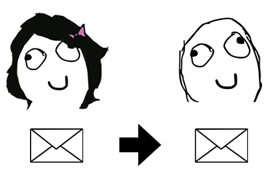
\includegraphics[height=2.5cm]{bilder/modell.jpg}
				\end{figure}
		\end{column}
		\begin{column}{7cm}	
			\centering
			\begin{itemize}	
				\item Alice möchte Bob Nachricht senden
				\item Normal: Schutz des Inhalts
				\item Jetzt: Schutz der Identitäten
			\end{itemize}
		\end{column}
	\end{columns}
	\end{exampleblock}
	}
	
	\invisible<1> {
	\begin{alertblock}{Angreifer Eve möchte Ziele gefährden}
		\begin{columns}[T]
		\begin{column}{2.5cm}
				\vspace{-.3cm}
				\begin{figure}
					
\includegraphics[height=2.5cm]{bilder/eve.jpg}
				\end{figure}
		\end{column}
		\begin{column}{7cm}
			\begin{itemize}	
				\item Netzwerk beobachten
				\item Einsicht in Traffic
				\item Pakete abfangen, senden, manipulieren und senden
			\end{itemize}
		\end{column}
	\end{columns}
	\end{alertblock}
	}

\end{frame}

\section{Cypherpunk-Remailer}
\begin{frame}
	\frametitle{Cypherpunk-Remailer}
	\begin{block}{Wesentliche Eigenschaften}
		\begin{itemize}
			\item Klassifizierung: Typ-I Remailer
			\pause
			\item "Cipher", "Cyber", "Punk"
			\pause
			\item Anonymisierend
			\pause
			\item Inspiration: Mix-Netzwerke \textit{(David Chaum)}
			\pause
			\item E-Mail Protokoll
		\end{itemize}
	\end{block}
\end{frame}

\begin{frame}
	\frametitle{Cypherpunk-Remailer}
	\begin{block}{Basis des Protokolls}
		Netzwerk von mehreren verschiedenen Cypherpunk-Remailern
	\end{block}
	\begin{columns}[T]
		\begin{column}[T]{5cm}
			\begin{center}
			Cypherpunk-Remailer \(C\) \\   

			\begin{figure}
			
\includegraphics[height=3cm]{bilder/remailer.eps}
			\end{figure}
			\end{center}
		\end{column}
		\begin{column}[T]{5cm}
			\begin{center}	
			\begin{itemize}
				\item öffentlicher Schlüssel \(D_{C}\)
				\item privater Schlüssel \(E_{C}\)
				\item Nachricht entschlüsseln und weiterleiten
				\item Nachrichten-Header modifizieren
			\end{itemize}	
			\end{center}
		\end{column}
	\end{columns}
\end{frame}

\subsection{Funktionsweise}
\begin{frame}
	\frametitle{Cypherpunk-Remailer - Vorbereitung}
	\begin{block}{Alice kennt:}
		\begin{itemize}
			\item Remailer-Netzwerk \(C_1, C_2, ..., C_n\)
			\item öffentliche Schlüssel \(E_{C_1}, E_{C_2}, ..., E_{C_n}\)
		\end{itemize}	
	\end{block}

	\begin{block}{Alice muss}
	\begin{itemize}
		\item Auswahl Remailer
		\item Reihenfolge bestimmen
	\end{itemize}	
	\end{block}

	\begin{exampleblock}{Ziel}
		Nachricht wird über Pfad an Bob gesendet
	\end{exampleblock}	
\end{frame}

\begin{frame}
	\frametitle{Cypherpunk-Remailer - Vorbereitung}
	\begin{block}{Inhalt einer Nachricht}	
		\begin{itemize}	
			\item Adresse \(A\)
			\item Nachricht \(N\)
		\end{itemize}	
	\end{block}	
	\begin{block}{schichtenweise Verschlüsselung}	
		\begin{equation}
			N' = (A_1, E_{C_1}(A_2, E_{C_2} (... (A_n,  E_{C_n}(A_{Bob}, E_{Bob}(N)))
		\end{equation}	
	\end{block}	

	\begin{exampleblock}{Beispiel}	
		\begin{center}
		\begingroup
			\setbox0=\hbox{
				
\includegraphics[height=1cm]{bilder/nachricht_bob.jpg}}%
			\parbox{\wd0}{\box0}
		\endgroup
		\hspace{0.1cm}
		$\rightarrow$
		\hspace{0.1cm}
		\begingroup
			\setbox0=\hbox{
				
\includegraphics[height=1cm]{bilder/nachricht_cn.jpg}}%
			\parbox{\wd0}{\box0}
		\endgroup
		\hspace{0.1cm}
		$\rightarrow$ \hspace{0.1cm} (...)
		\hspace{0.1cm}
		$\rightarrow$
		\hspace{0.1cm}
		\begingroup
			\setbox0=\hbox{
				
\includegraphics[height=1cm]{bilder/nachricht_c2.jpg}}%
			\parbox{\wd0}{\box0}
		\endgroup
		\hspace{0.1cm}
		$\rightarrow$
		\hspace{0.1cm}
		\begingroup
			\setbox0=\hbox{
				
\includegraphics[height=1cm]{bilder/nachricht_c1.jpg}}%
			\parbox{\wd0}{\box0}
		\endgroup
		\end{center}
	\end{exampleblock}	
\end{frame}

\begin{frame}
	\frametitle{Cypherpunk-Remailer - Ablauf}
	\begin{block}{Ablauf Sendevorgang}
		\begin{itemize}
			\item Alice sendet N' an \(C_1\)
			\item \(C_1\) erhält \(A_2\) und verschlüsselte Nachricht
			\item \(C_1\) sendet Nachricht an Adresse in \(A_2\)
			\item \(C_2\) erhält \(A_3\) und verschlüsselte Nachricht
			\item \((...)\)
			\item \(C_n\) sendet Nachricht an Adresse von Bob
		\end{itemize}	
	\end{block}
\end{frame}

\begin{frame}
	\frametitle{Cypherpunk-Remailer}
	\begin{exampleblock}{Was haben wir erreicht?}	
		\begin{itemize}	
			\item \(C_x\) kennt nur unmittelbaren Nachfolger und Vorgänger
			\item Bob kennt nur letzten Remailer
			\item Alice kennt als Einzige gesamten Pfad
		\end{itemize}	
	\end{exampleblock}
	\begin{center}
		und 
\includegraphics[height=2cm]{bilder/eve.jpg} ?
	\end{center}			
\end{frame}	

\subsection{Sicherheitsanalyse}
\begin{frame}
	\frametitle{Cypherpunk-Remailer - Sicherheitsanalyse}
	\begin{alertblock}{Traffic Analyse}	
		\begin{itemize}	
			\item Nachrichtengröße
			\item leitet Nachrichten sofort weiter
		\end{itemize}	
	\end{alertblock}

	\begin{alertblock}{Replay Angriff}	
		\begin{itemize}	
			\item Eve kann Nachrichten abfangen und wieder einspielen
			\item Duplikate werden nicht erkannt
		\end{itemize}	
	\end{alertblock}

	\begin{columns}[T]
		\begin{column}[T]{5cm}
			\begin{center}
				
\includegraphics[height=3cm]{bilder/alice_sad.jpg}
			\end{center}
		\end{column}
		\begin{column}[T]{5cm}
			\begin{center}	
				
\includegraphics[height=3cm]{bilder/eve.jpg}
			\end{center}
		\end{column}
	\end{columns}	
\end{frame}

\subsection{Zuverlässigkeitsanalyse}
\begin{frame}
	\frametitle{Cypherpunk-Remailer - Zuverlässigkeit}
	\begin{alertblock}{Remailer im Pfad fällt aus}	
		\begin{itemize}	
			\item Jeder Remailer kennt nur unmittelbaren Nachfolger und Vorgänger
			\item Nachricht verschwindet
			\item Fehler bleibt unbemerkt
		\end{itemize}	
	\end{alertblock}


	\begin{columns}[T]
		\begin{column}[T]{5cm}
			\begin{center}
				
\includegraphics[height=3cm]{bilder/alice_sad.jpg}
			\end{center}
		\end{column}
		\begin{column}[T]{5cm}
			\begin{center}	
				
\includegraphics[height=3cm]{bilder/bob_sad.jpg}
			\end{center}
		\end{column}
	\end{columns}	
\end{frame}

\section{Mixmaster-Remailer}

\begin{frame}
	\frametitle{Mixmaster-Remailer - Motivation}
	\begin{itemize}
		\item Baut auf Cypherpunk-Remailer auf
		\item Basis: "Mixmaster and remailer attacks" (Lance Cottrell)
		\begin{itemize}	
			\item deckt Sicherheitsschwächen auf
			\item bietet Lösungsansätze
		\end{itemize}
	\end{itemize}

	\begin{exampleblock}{Ziel}
		\centering
		Weiterentwicklung des existierenden Protokolls, um Sicherheitslücken zu schließen.
	\end{exampleblock}
\end{frame}

\subsection{Funktionsweise}
\begin{frame}
	\frametitle{Mixmaster-Remailer - Funktionsweise}
	\visible<1-2>{
		\begin{block}{Was bleibt gleich?}
			\begin{itemize}
				\item Remailernetzwerk
				\item schichtenweise Verschlüsselung
				\item E-Mail Protokoll 
			\end{itemize}
		\end{block}
	}
	
	\invisible<1>{
		\begin{alertblock}{Ausblick: Was muss sich ändern?}
			\begin{itemize}	
				\item Traffic transparent gestalten
				\item Zeitliche Zuordnung
				\item Duplikate erkennen
				\item Manipulierte Nachrichten erkennen
			\end{itemize}
		\end{alertblock}
	}
\end{frame}

\begin{frame}
	\frametitle{Mixmaster-Remailer - Chunks}
	\begin{exampleblock}{Ziel}
		Traffic transparent gestalten
	\end{exampleblock}

	\begin{itemize}	
		\item Nachricht in gleich große Chunks aufteilen
		\item Auffüllen mit zufälligen Dummy-Daten
		\item Chunks statt Nachricht über Netzwerk verteilen
		\item Jeder Chunk (möglichst) auf verschiedenem Pfad
		\begin{itemize}
			\item letzter Remailer im Pfad
			\item Zusammensetzung
			\item Weiterleitung
		\end{itemize}	
	\end{itemize}	
\end{frame}

\begin{frame}
	\frametitle{Mixmaster-Remailer - Pool}
	\visible<1-2>{
	\begin{exampleblock}{Ziel}
		Zeitliche Zuordnung
	\end{exampleblock}

	\begin{itemize}	
		\item Einkommende Nachrichten sammeln
		\item beliebige Größe
		\item zufällige Reihenfolge
	\end{itemize}
	}	

	\invisible<1> {
	\begin{alertblock}{Pool wird nie voll?}
		\begin{itemize}
			\item individueller Zeitpunkt
			\item zufallsgenerierte Dummy-Nachrichten
		\end{itemize}
	\end{alertblock}
	}
\end{frame}

\begin{frame}
	\frametitle{Mixmaster-Remailer - Integrität}
	\begin{exampleblock}{Ziel}
		Duplikate und Manipulation
	\end{exampleblock}

	\begin{block}{Signatur}
		\begin{itemize}	
			\item Erkennung von manipulierten Nachrichten
			\item werden verworfen
		\end{itemize}
	\end{block}

	\begin{block}{Identifikation}
		\begin{itemize}
			\item verschlüsselte ID
			\item Duplikate werden erkannt
			\item werden verworfen
		\end{itemize}
	\end{block}
\end{frame}

\begin{frame}
	\frametitle{Mixmaster-Remailer - Ablauf}
	\begin{itemize}
		\item Alice benötigt Client-Software
		\item Nachricht wird aufgeteilt
		\item Chunks werden über das Netzwerk weitergeleitet
		\item letzter Remailer sammelt Chunks
		\item entfernt evtl. Dummy-Daten
		\item setzt Nachricht zusammen und leitet an Bob	
	\end{itemize}
\end{frame}

\subsection{Analyse}
\begin{frame}
	\frametitle{Mixmaster-Remailer - Sicherheitsanalyse}
	\begin{exampleblock}{Traffic Analyse}
		\begin{itemize}
			\item einheitliche Nachrichtengröße
			\item keine zeitliche Zuordnung
			\item konstanter Traffic-Level
		\end{itemize}
	\end{exampleblock}

	\begin{exampleblock}{Replay Angriff}
		\begin{itemize}
			\item Duplikate werden erkannt und ignoriert
			\item Manipulationen werden erkannt und ignoriert
		\end{itemize}
	\end{exampleblock}

	\centering
	
\includegraphics[height=2cm]{bilder/alice.jpg} ?
\end{frame}

\begin{frame}
	\visible<1-2>{
	\frametitle{Mixmaster-Remailer - Sicherheitsanalyse}
	\begin{alertblock}{Angriffsmöglichkeit}
		\begin{itemize}
			\item Nachricht von Alice abfangen und zurückhalten
			\item Überflütung des Remailernetzwerks mit eigenen Nachrichten
			\item Keine anderen Nachrichten außer Eves mehr im Netzwerk
			\item Einspielen von Alice Nachricht
			\item Empfänger dieser Nachricht muss Bob sein
		\end{itemize}
	\end{alertblock}
	}

	\invisible<1>{
	\centering
	Aber:
	\begin{columns}[T]
		\begin{column}[T]{5cm}
			\begin{center}
				
\includegraphics[height=2.5cm]{bilder/alice.jpg}
			\end{center}
		\end{column}
		\begin{column}[T]{5cm}
			\begin{center}	
				
\includegraphics[height=2.5cm]{bilder/eve_sad.jpg}
			\end{center}
		\end{column}
	\end{columns}	
	}	
\end{frame}

\section{Nym-Server}

\begin{frame}
	\frametitle{Nym-Server - Motivation}
	\begin{itemize}
		\item bisher - Anonymisierung
		\begin{itemize}	
			\item Identität ist verborgen
			\item Bob kennt nur letzten Remailer
			\item antworten nicht möglich
		\end{itemize}
		\pause
		\item nun - Pseudonymisierung
		\begin{itemize}	
			\item Identität versteckt hinter Decknamen
			\item Bob kennt Decknamen
			\item antworten möglich
		\end{itemize}
	\end{itemize}

	\pause
	Typ-0 Remailer?
	\pause

	\begin{block}{Definition (Quelle - techopedia.com)}
		A nym server is a pseudonym server that furnishes an untraceable email address. The purpose of this server is to allow users to have usernames (pseudonyms) and send and 			receive messages without revealing their true identities.
		Even the nym server operators cannot trace a user's email address.
	\end{block}
\end{frame}

\begin{frame}
	\frametitle{Nym-Server - Umsetzung}

	\begin{block}{Ziele}
		\begin{itemize}
			\item Schicken und Empfangen über Pseudonym
			\item Betreiber transparent für Betreiber
		\end{itemize}
	\end{block}

	\pause

	Idee: Umsetzung über Cypherpunk-Remailer
	
\end{frame}

\begin{frame}
	\frametitle{Nym-Server - Umsetzung}

	\begin{block}{Bestandteile eines Nyms}
		\begin{itemize}
			\item öffentlicher Schlüssel
			\item Reply-Block
			\item Pseudonym
		\end{itemize}
	\end{block}

	\pause

	\begin{block}{Reply-Block}
		\begin{itemize}
			\item Enthält Pfad über Cypherpunk-Remailer Netzwerk zum Empfänger hinter dem Nym.
			\item schichtenweise verschlüsselt
		\end{itemize}
	\end{block}
\end{frame}

\begin{frame}
	\frametitle{Nym-Server - Ablauf (Erstellung)}

	\begin{itemize}
		\item Bob möchte Pseudonym
		\begin{itemize}
			\item sucht sich Menge an Cypherpunk-Remailern heraus
			\item erstellt Reply-Block
			\item denkt sich Pseudonym aus
			\item stellt öffentlichen Schlüssel bereit
		\end{itemize}
		\item schickt Nym an Nym-Server
		\item Achtung: Muss anonymisiert gesendet werden!
		\item (ggf. Validierung des Nyms vom Nym-Server)
	\end{itemize}
\end{frame}

\begin{frame}
	\frametitle{Nym-Server - Ablauf (Verwendung)}

	\begin{itemize}
		\item Alice 
		\begin{itemize}
			\item kennt Bobs Pseudonym
			\item möchte Bob eine Nachricht zukommen lassen
			\item schickt Nachricht an Bobs Pseudonym an den Nym-Server
		\end{itemize}

		\pause

		\item Nym-Server
		\begin{itemize}
			\item findet den Nym
			\item verschlüsselt Nachricht mit öffentlichem Schlüssel
			\item schickt Nachricht mit Reply-Block an ersten Remailer im Block
		\end{itemize}

		\item Nachricht von Alice wird über Remailernetzwerk an Bob geschickt
	\end{itemize}
\end{frame}

\begin{frame}
	\frametitle{Nym-Server}
	\centering
	Sicherheit?
\end{frame}

\section{Mixminion-Remailer}

\begin{frame}
	\frametitle{Mixminion - Motivation}
	
	\begin{itemize}
		\item Aktualität
		\item Nym-Server unsicher
		\item Zuverlässigkeit
	\end{itemize}
\end{frame}

\begin{frame}
	\frametitle{Mixminion - Umsetzung Übersicht}

	\begin{block}{Was bleibt gleich?}
		\begin{itemize}
			\item Netzwerkstruktur
			\item Anonymisierung
			\item Traffictransparenz
			\item schichtenweise Verschlüsselung (Header)
		\end{itemize}
	\end{block}

	\begin{block}{Was ist neu?}
		\begin{itemize}
			\item eigenes Protokoll
			\item verschlüsselte Verbindung (TLS)
			\item automatisches Remailerverzeichnis
			\item Antworten auf anonymisierte Nachrichten
		\end{itemize}
	\end{block}
\end{frame}

\begin{frame}
	\frametitle{Mixminion - Protokoll}

	\begin{columns}[T]
		\begin{column}{5cm}
			\begin{figure}
				\centering
				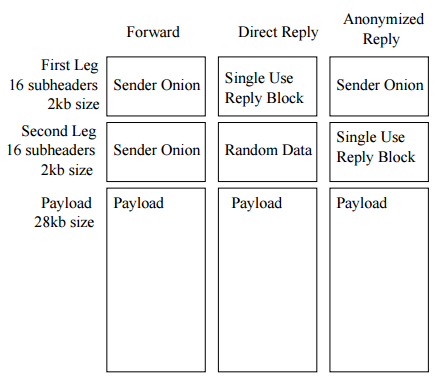
\includegraphics[height=5cm]{bilder/mixminion_messages.jpg}
			\end{figure}
		\end{column}
		\begin{column}{5cm}	
			\centering
			\begin{itemize}	
				\vspace{2cm}
				\item drei Typen
				\item Ununterscheidbarkeit
				\item zweigeteilter Header
			\end{itemize}
		\end{column}
	\end{columns}
\end{frame}

\begin{frame}
	\frametitle{Mixminion - normale Nachricht}

	\begin{columns}[T]
		\begin{column}{5cm}
			\begin{figure}
				\centering
				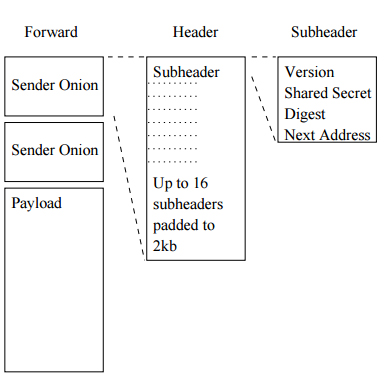
\includegraphics[height=5cm]{bilder/mixminion_standard.jpg}
			\end{figure}
		\end{column}
		\begin{column}{5cm}
			\begin{block}{Subheader}	
				\begin{itemize}	
					\item Master-Secret für TLS
					\item Adresse des nächsten Remailers (verschlüsselt)
					\item Prüfsumme zur Überprüfung restlichen Headers
				\end{itemize}
			\end{block}
		\end{column}
	\end{columns}
\end{frame}


% Reply Erklären
% Inhalt von SURB erläutern
% Warum Random-Data?
% Payload = Antwortnachricht
\begin{frame}
	\frametitle{Mixminion - einfache Antwort}

	\begin{columns}[T]
		\begin{column}{3cm}
			\begin{figure}
				\centering
				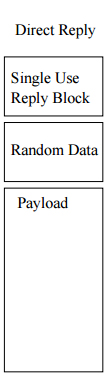
\includegraphics[height=5cm]{bilder/mixminion_reply.jpg}
			\end{figure}
		\end{column}
		\begin{column}{7cm}
			\vspace{1cm}
			\begin{block}{SURB}	
				\begin{itemize}	
					\item Adresse von Alice (verschlüsselt)
					\item Pfad durch das Netzwerk (verschlüsselt)
					\item nur einmal verwendbar
					\item von Bob nicht entschlüsselbar
				\end{itemize}
			\end{block}
		\end{column}
	\end{columns}
\end{frame}

%% neue Folie nur mit Bild
% Anonym. Reply erklären
% Wozu Sender-Onion hier?
\begin{frame}
	\frametitle{Mixminion - anonyme Antwort}

	\begin{columns}[T]
		\begin{column}{3cm}
			\begin{figure}
				\centering
				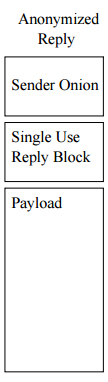
\includegraphics[height=5cm]{bilder/mixminion_anonreply.jpg}
			\end{figure}
		\end{column}
		\begin{column}{7cm}
				\vspace{2cm}
				\begin{itemize}	
					\item Pfad von Bob durch Netzwerk
					\item SURB von Alice
					\item Ziel: Auch Bob bleibt anonym.
				\end{itemize}
		\end{column}
	\end{columns}
\end{frame}

% Verzeichnisserver
% Aufzählung was er beinhaltet
% Ablauf erklären
% was machen VZ-Server?
% wie kriegen sie Remailerdaten?
\begin{frame}
	\frametitle{Mixminion - Verzeichnisserver}

	\begin{block}{Verzeichnisserver}
		\begin{itemize}
			\item aktuell verwendete Schlüssel des Remailers
			\item aktuellen Zustand
			\item die Existenz eines Remailers
		\end{itemize}
	\end{block}

	\begin{itemize}
		\item redundante Gruppe von Servern
		\item regelmäßige Kommunikation
		\begin{itemize}
			\item untereinander (Verifikation)
			\item Remailer (Synchronisation)
		\end{itemize}
	\end{itemize}
\end{frame}

\begin{frame}
	\frametitle{Mixminion - Ablauf}
	
	\begin{itemize}
		\item Alice besorgt sich aktuelle Informationen über Verzeichnisserver (Schlüssel, Adresse von Mix)
		\item Aufbereitung der Nachricht gemäß Protokoll
		\item Alice schickt Nachricht an ersten Remailer
		\item Jeder Remailer:
		\begin{itemize}
			\item Prüft Integrität des Headers (Prüfsumme)
			\item Speichert Prüfsumme (Replay-Angriff) bis Schlüsseltausch
			\item TLS-Verbindung zum nächsten Remailer (verifiziert und verschlüsselt)
			\item überträgt Nachricht
		\end{itemize}
		\item \textbf{swap-Operation}
		\item danach weiter bis Bob Nachricht erhält
	\end{itemize}
\end{frame}

% Sicherheitsanalyse
% theoretisch sicher
% praktisch? -> unbekannt, Implemetierung nie über beta hinausgekommen. keine Praxiserfahrung vorhanden.
\begin{frame}
	\frametitle{Mixminion - Sicherheitsanalyse}	
	\centering
	Sicherheit?

	\begin{columns}[T]
		\visible<1-2>{
		\begin{column}{5cm}
			\begin{figure}
				\centering
				
\includegraphics[height=5cm]{bilder/mixminion_theorie.jpg}
			\end{figure}
		\end{column}
		}

		\invisible<1>{
		\begin{column}{5cm}\begin{figure}
				\centering
				
\includegraphics[height=5cm]{bilder/mixminion_praxis.jpg}
			\end{figure}
		\end{column}
		}
	\end{columns}
\end{frame}






\end{document}